\documentclass[UTF-8]{ctexart}
\usepackage{geometry}
\usepackage{verbatim}
\usepackage{amsmath}
\usepackage{amsthm}
\usepackage{listings}
\usepackage{graphicx}
\usepackage{color}
\usepackage{stmaryrd}

\newtheorem{proposition}{Proposition}
\author{李勰 201928015029029}
\title{形式化方法大作业}
\date{\today}


\geometry{a4paper, scale = 0.8}
\begin{document}
\maketitle

\begin{enumerate}
\item 第一题:对各种模型和分量进行阐述,并且说明要素在系统建模中起到的作用。
以下按照模型依次讨论和解释。
\begin{itemize}
\item Kripke模型:

A Kripke structure is a tuple: $\langle S, R, I\rangle$. 其中$S$表示状态的集合,$R$表示迁移关系,$I$是初始状态的集合。对于一个信息系统来说,状态的集合里的状态指的是变量的赋值,例如对于软件系统来说,变量是什么值,对于计算机系统,还包括寄存器的状态,PC的值等等。$R$表示可能的状态之间的迁移关系,比如一个If语句,如果guard成立,做一个迁移,如果不成立做另外一个迁移。初始状态集$I$表示系统最初的可能的状态。


\item 公平Kripke模型

和Kripke模型相比,公平的Kripke定义为$\langle S,R,I,F\rangle$,多了一个$F$,表示公平性约束的有穷集合。这里直观上来说公平的意思就是,对于$F$里面的每个状态,我的一个计算的序列,如果是无穷长度的序列,必须无穷次经过其中每一个状态。如果把$\pi$看作一个模型上的路径的话,可以写为$\inf(\pi)\cap f \ne \emptyset$.公平性在实际系统建模的刻画中,可以用来描述一些公平约束,例如两个进程不停对于一个资源的访问。我们要求其中每一个进程都能访问互斥资源无穷多次,就可以利用这个模型来建模。

\item 标号Kripke模型

标号Kripke模型是一个四元组$\langle S,R,I,L\rangle$,和Kripke模型相比多了个$L$,$L$的定义是从状态到原子命题集合的幂集的一个函数。这里的原子命题,引入了命题逻辑中的一些内容。主要的想法是,如果每个状态我们都能用$L$表示一些在该状态为真的原子命题,我们就能用逻辑更好的讨论该状态或者说模型的执行的过程中的性质。用这个模型我们可以很容易的从数学上表示出,对于所有执行$x$的值不等于$0$这样的性质。

\item 公平标号Kripke模型

该模型是以上两个模型的是原子命题集合$AP$上的$\langle S,R,I,L,F\rangle$五元组。这里不同的是$F$变为了公平性约束的有穷集合,也就是一个命题逻辑公式的集合。

\item 卫式迁移模型:

卫式迁移模型是对于一阶逻辑的一个扩充,卫式迁移模型的迁移是$\rightarrow,:=$共同定义的,比如$\phi \rightarrow \vec{x} = \vec{a}$. 直观上说就是如果公式$\phi$在状态上被满足,那么可以更新状态,这里的状态就是一个变量的赋值函数。卫式迁移模型和Kripke模型在语义上来说是等价的,同样的我们也有公平卫式迁移模型等模型。

\item 流程图模型

流程图模型是对卫式迁移模型的扩充,增加了两个集合的符号,辅助符号集合和标号符号集合$H,LB$. 语法上添加了分支和跳转,语义上和卫式迁移模型等价。

\item LTS模型

标号迁移模型,标号迁移模型是对Kripke模型的一个扩展,主要扩展了迁移时候的标号的有穷集合$\Sigma$,迁移的边上现在需要有个标号的guard。该类模型的主要作用是对实时系统做建模,其中$\Sigma$所代表的guard就表示了系统和外界环境做交互时,可能收到的动作字母表。

双标号迁移模型,同时有$\Sigma,L$的Kripke模型。

\item B\"uchi自动机

B\"uchi自动机是$\omega$-自动机中的一种,定义和DFA类似,只不过$\omega$-自动机讨论的输入字符串是$\Sigma^\omega$之中的无穷串,输入串接受当且仅当至少有一个$F$中的接收状态在输入串上出现无穷多次。B\"uchi自动机结合LTL或者CTL在模型检验中有重要的作用。此外,还有多种$\omega$自动机,他们的定义和接收条件如下:
\begin{itemize}

\item GNBA: $F$是状态集合的集合,字符串为接收当且仅当他上面出现的无穷次的字符集合和$F$中每个集合的交不为空。

\item Muller: $F$是状态集合的集合,字符串为接收当且仅当他上面出现的无穷次的字符集合$f$和$F$中的某个集合相等。

\item Streett: $F$是状态集合对的集合,字符串为接收当且仅当他上面出现的无穷次的字符集合和$(f,g)\in F$中的$f$的交不为空,可以推出他和$g$的交也不为空。

\item Rabin:$F$是状态集合对的集合,字符串为接收当且仅当他上面出现的无穷次的字符集合和$(f,g)\in F$中的$f$的交不为空,可以推出他和$g$的交为空。

\item Parity: $F$是状态集合到自然数的映射,字符串为接收当且仅当无穷出现的状态中的的映射最小值为偶数。

\end{itemize}


\item 时间自动机/时间迁移系统

时间自动机是一个五元组$\langle \Sigma, S,X,\Delta, I\rangle$. 其中$X$是时间变量的集合,迁移的定义是$\Delta \subseteq S\times \Sigma \times 2^X \times \Phi(X) \times S$. 表示在做迁移的时候,首先要求读到的字符相同,并且对于时间变量的约束$\Phi(X)$满足,在这样的情况下我们进行迁移,并且将$X$中的某个子集的时钟值更新为$0$.这样的模型可以用于建模和事件相关的系统,比如程序中有个计时器,会随着程序的运行重置、增大等。

\item Hybrid自动机

Hybrid自动机是一个六元组$\langle \Sigma, S, X, \Delta, I, flow\rangle$. $X$ 为实数变量的集合,$flow$是从$S$到$\Phi(X\cup X)$上的映射。Hybrid自动机的状态空间是,状态集合和赋值函数集合的笛卡尔积。

\end{itemize}


\item 第二题:对各种模型的各类性质包括正确性的概念和时序逻辑性质的描述方法以及对这些性质进行验证的各种方法的基本思想和提高效率的考虑方面进行阐述。

对性质进行阐述,我们这里考虑对模型进行分类,并且给出不同类型的序列的相应性质的定义,如果有算法进行阐述。此外第二部分将给出LTL和CTL的定义,在定义的基础上给出验证方法。

\begin{itemize}
\item 性质

在讨论模型的时候我们通常会研究模型上的计算的性质,在形式化方法中,我们经常考虑的基础的性质有。可达性、安全、公平、必达、可避免等性质。通过研究系统的这些性质,我们可以将我们感兴趣的性质写出来,并用相关算法分析系统是否满足或者违反这些性质,从而得到这个系统的重要信息。

\begin{itemize}
\item Kripke模型的性质:

对于状态子集$A$的可达性质,可达性质可以利用模型对应的有向图模型做遍历,分析一个性质是否是可达性质。此外还可以用不动点的方式寻找这样的可达性质。

安全性质$A$,表示所有的计算都是$A$计算,也就是$\neg A$是不可达性质。安全性质的分析也是类似,考虑$\neg A$,在模型图上做搜索和遍历,如果遍历到某个状态是$\neg A$的状态,说明安全性质被违反,否则是$A$安全的。

可避免性质$A$,等价于$\neg$是可达性质,也就是存在$\neg A$的计算。可避免性质的分析,可以在图上考虑满足$\neg A$的强连通分量,如果存在从$\neg A$状态到这样的强连通分量的有穷路径,说明我们可以找到一个这样的强连通分量使得计算可以呆在这个SCC中,从而避免$A$.

必达性质,必达性质是可避免性质的反面,如果没有找到可避免性质中那样的强连通分量,那么性质$A$为必达性质。

\item 公平Kripke模型

讨论公平Kripke模型的性质,我们需要先确定什么是公平路径。公平路经指的是,如果对于一条路径$\pi$,它上面出现的无穷次的状态集合为$\inf(\pi)$,那么路径$\pi$是公平的当且仅当无穷出现的无穷次的状态集合和$F$中的每个集合的交集不为空。

公平可达性质:$A$称为$K$模型的公平可达性质,当且仅当$K$中有能到达$A$中状态的公平路径。公平可达性质的分析,首先先看那些$A$中的状态是公平状态,在用遍历的算法看是否能从初始状态可达。

公平安全性质,公平可避免性质,公平必达性质的定义和公平可达性质的定义类似,都是要加上对计算的公平性的约束。其分析方法和Kripke模型类似,都是需要对之前考虑的SCC或者状态集合加上公平性的约束。

\item 卫式迁移模型的性质

卫式迁移模型的计算是一个变量到值的函数的序列。

安全性性质:如果$\phi$是一个安全性质,当且仅当卫式迁移模型的所有计算都是$\phi$计算。

必达性质:如果是必达性质,表示所有计算都能到达必达性质的状态。

公平卫式迁移模型,同样有着公平安全性之和公平必达性质的定义。

\item 流程图模型 \& 程序化结构模型

这两类模型通常用来模拟程序的流程,因此考虑的性质也是程序的基本性质,例如中执行,部分正确性和完全正确性。

终止性表示程序最终会停止。部分正确性指程序如果终止,那么结果一定正确。完全正确性是终止性和部分正确性合起来。这些性质在基于模型的验证和推理证明中都有详细的应用。比如程序的终止性,我们可以用模型检验来做,也可以用寻找秩函数的方式来做。程序的部分正确行,可以用Hoare‘s Logic推理证明,也可以用基于LTL的模型检验算法证明等等。



\end{itemize}

\item 时序逻辑


\begin{itemize}

\item 基于时序逻辑性质的描述和验证方法

时序逻辑主要有LTL和CTL两种。这两种时序逻辑可以用来描述系统的时序性质,并且利用这些时序逻辑公式和迁移模型或者自动机,对系统的性质进行验证。

线性时序逻辑:线性时序逻辑的模型是一个LTS和一个无穷路径$\pi$.和命题逻辑比起来,时序逻辑主要多出了两个操作符$\textbf{X}$和$\textbf{U}$, $\textbf{X}$表示Util和Next的语义,表示对于一条路径上的状态的时序性质的约束。

利用LTL来做验证最基本的算法是用B\"uchi自动机做验证,具体的思路就是,存在从LTL到B\"uchi自动机的算法,使得自动机接受的无穷字符串都满足LTL公式。如果我们想要验证一个性质$\phi$,那么我们可以用算法获取$\neg \phi$的B\"uchi自动机,用表示系统的自动机$B$和自动机做交,并判断自动机的语言是否为空。如果为空,说明系统满足我们希望验证的性质,如果不为空,那么就可以找到系统中的一个违背性质的执行,作为反例。

计算树逻辑:计算树逻辑和LTL相比多出了\textbf{A}和\textbf{E}语法符号。和LTL不同,这里的计算树逻辑的模型是一颗树,表示计算的可能的过程,CTL中我们区分状态公式和路径公式,\textbf{A}和\textbf{E}后面都是路径公式。\textbf{A}表示从目前的这个状态开始,对于所有可能的路径都要满足某个路径性质,而\textbf{E}表示路径性质满足的存在性。此外我们还可以对迁移系统定义CTL的语义,可以用来做验证。

利用CTL来做模型检验的基本算法思想就是,可以把系统建模成迁移系统,用我们关心的性质$\phi$可以递归地找出满足公式$\phi$的状态集合,并且看迁移系统的初始状态是否在这个状态集合中,如果在状态集合中,我们可以认为系统满足我们考虑的性质。

\end{itemize}
\end{itemize}


\item 问题三:

1. 对流程设计建模,并且给出分量解释。

2.在两个不同模型的基础上,根据模型不同,应用算法证明正确性。

3. 讨论等价性,对验证方法进行讨论和比较。
\begin{enumerate}
\item 

第一种建模:用结构化程序建模

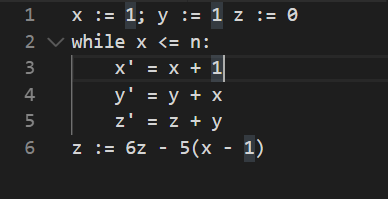
\includegraphics[scale=0.7]{1.PNG}

第二种建模:卫式迁移模型

$true \longrightarrow (x, y, z) := (1,1,0)$

$x \le n \longrightarrow (x, y, z) := (x+1, y+x, z+y)$

$\neg (x \le n) \longrightarrow (x, y, z) := (x, y, 6z - 5(x - 1))$



\item 
证明第一种建模的完全正确性可以利用秩函数证明终止性和和找到循环不变式并利用求最弱前置条件来证明。

第二种建模的完全正确性可以将$x = n^3$设为模型的必达性质,并写出表示正确性的公式,将公式扔给Z3求解器求解。


\item 流程图模型和卫式迁移模型之间式等价的。在课件中也有此等价性证明。从卫式迁移模型到流程图模型的证明较为简单。从流程图到卫式迁移模型的证明思路是,用PC = l和相应的变量更新表示等价。

课件中还证明了结构化程序建模和流程图式等价的,主要思路式因为流程图中的if语句和状态实际上可以表达出while循环的语义。

\end{enumerate}



\item 问题四:

\begin{enumerate}
\item CTL性质的模型检验算法如下
\begin{center}
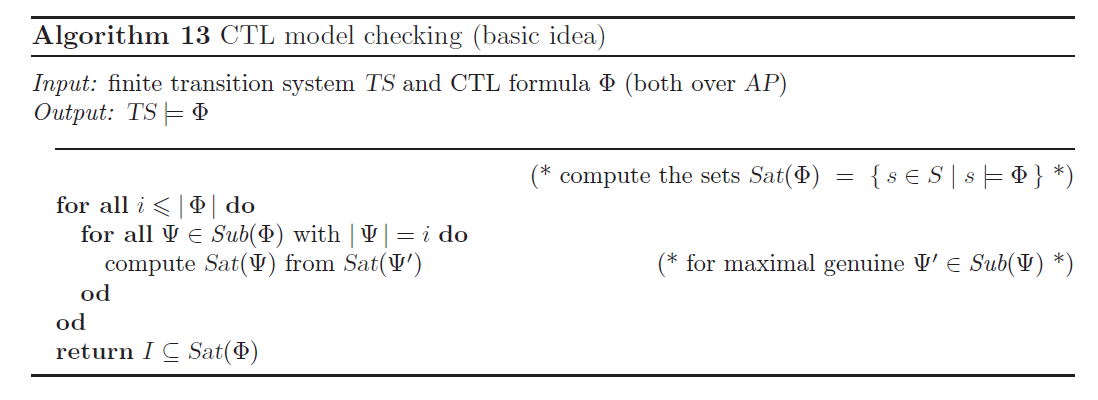
\includegraphics[scale=0.4]{2.PNG}

\end{center}
第一个性质:


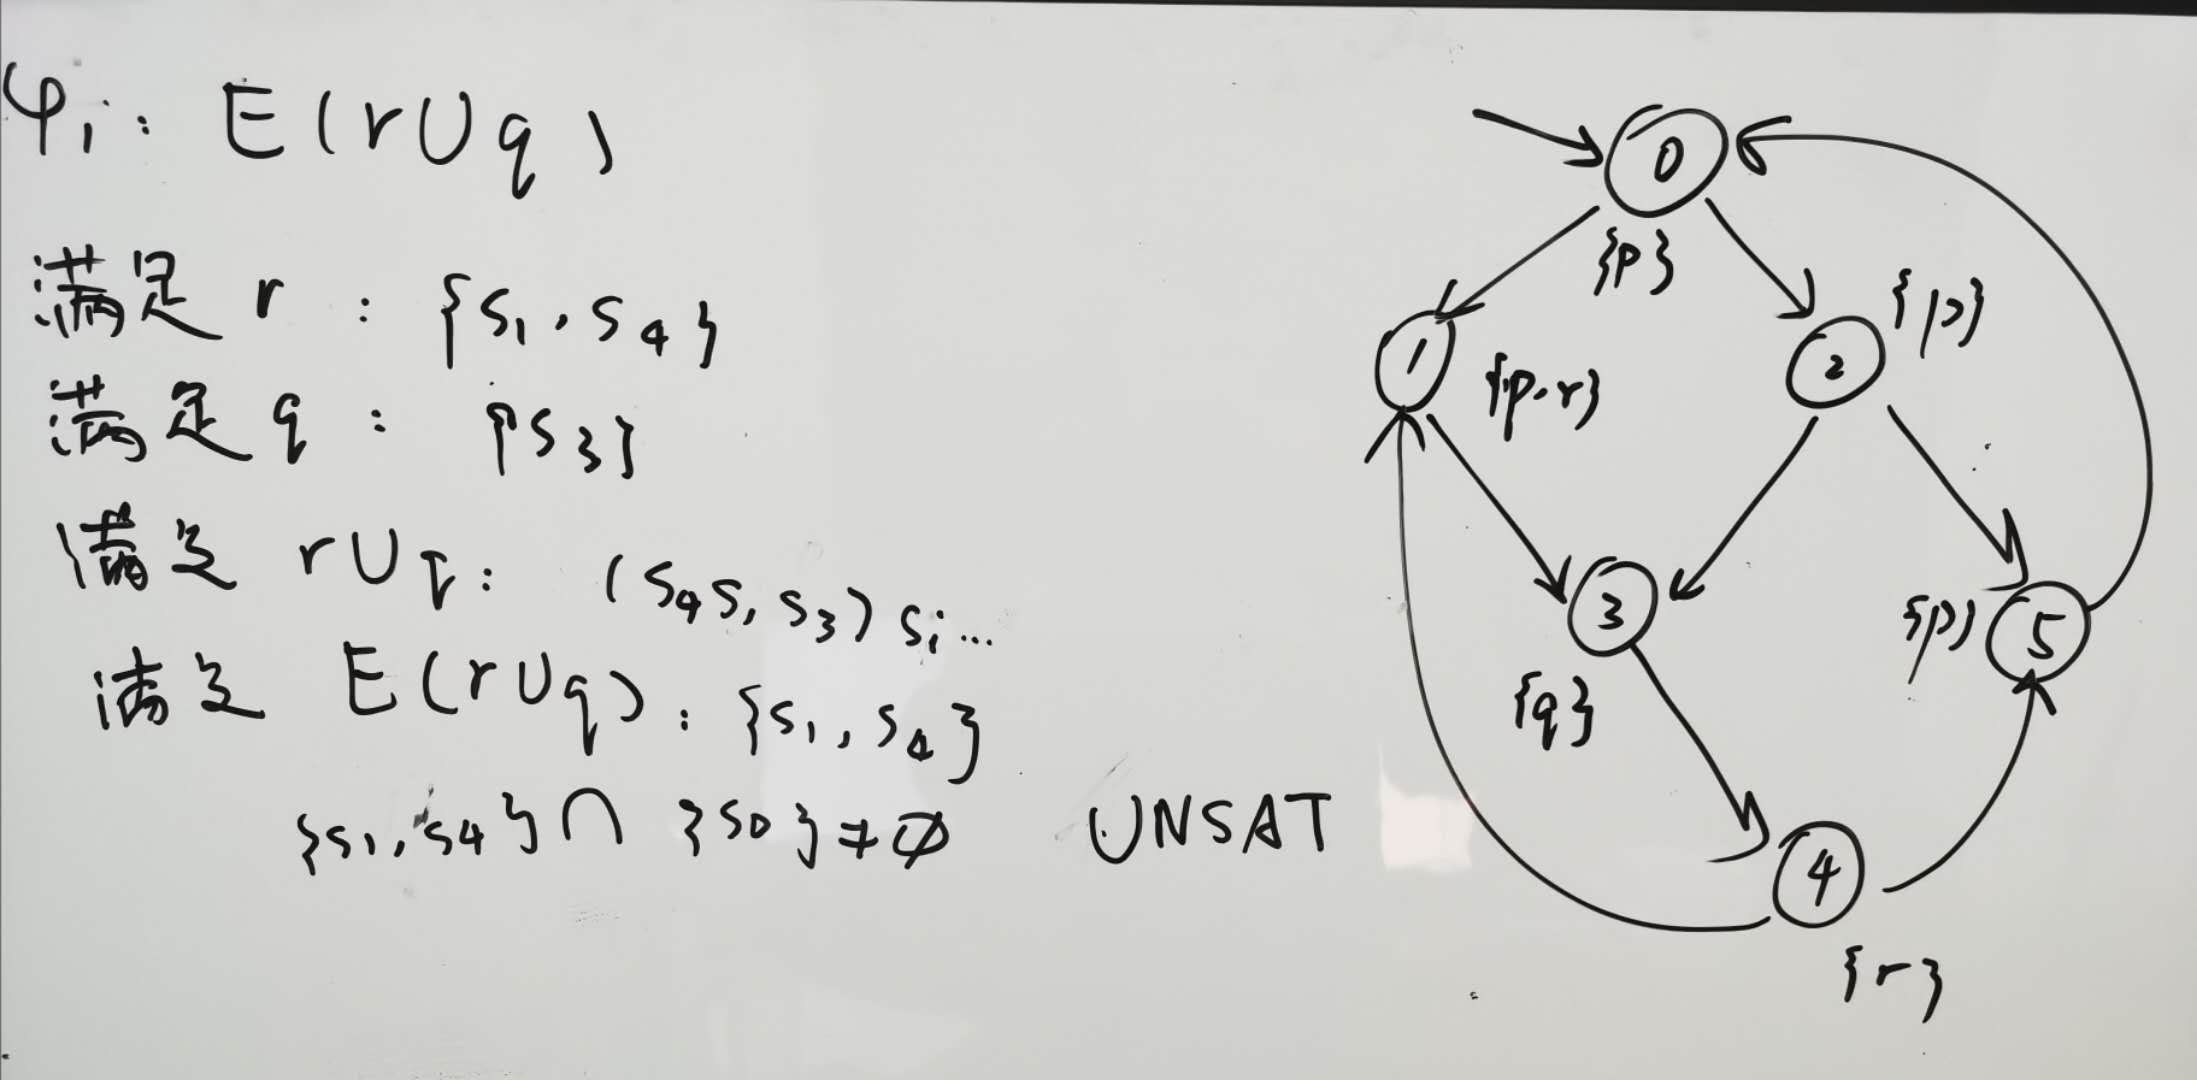
\includegraphics[scale= 0.12]{6.jpg}

第二个性质:


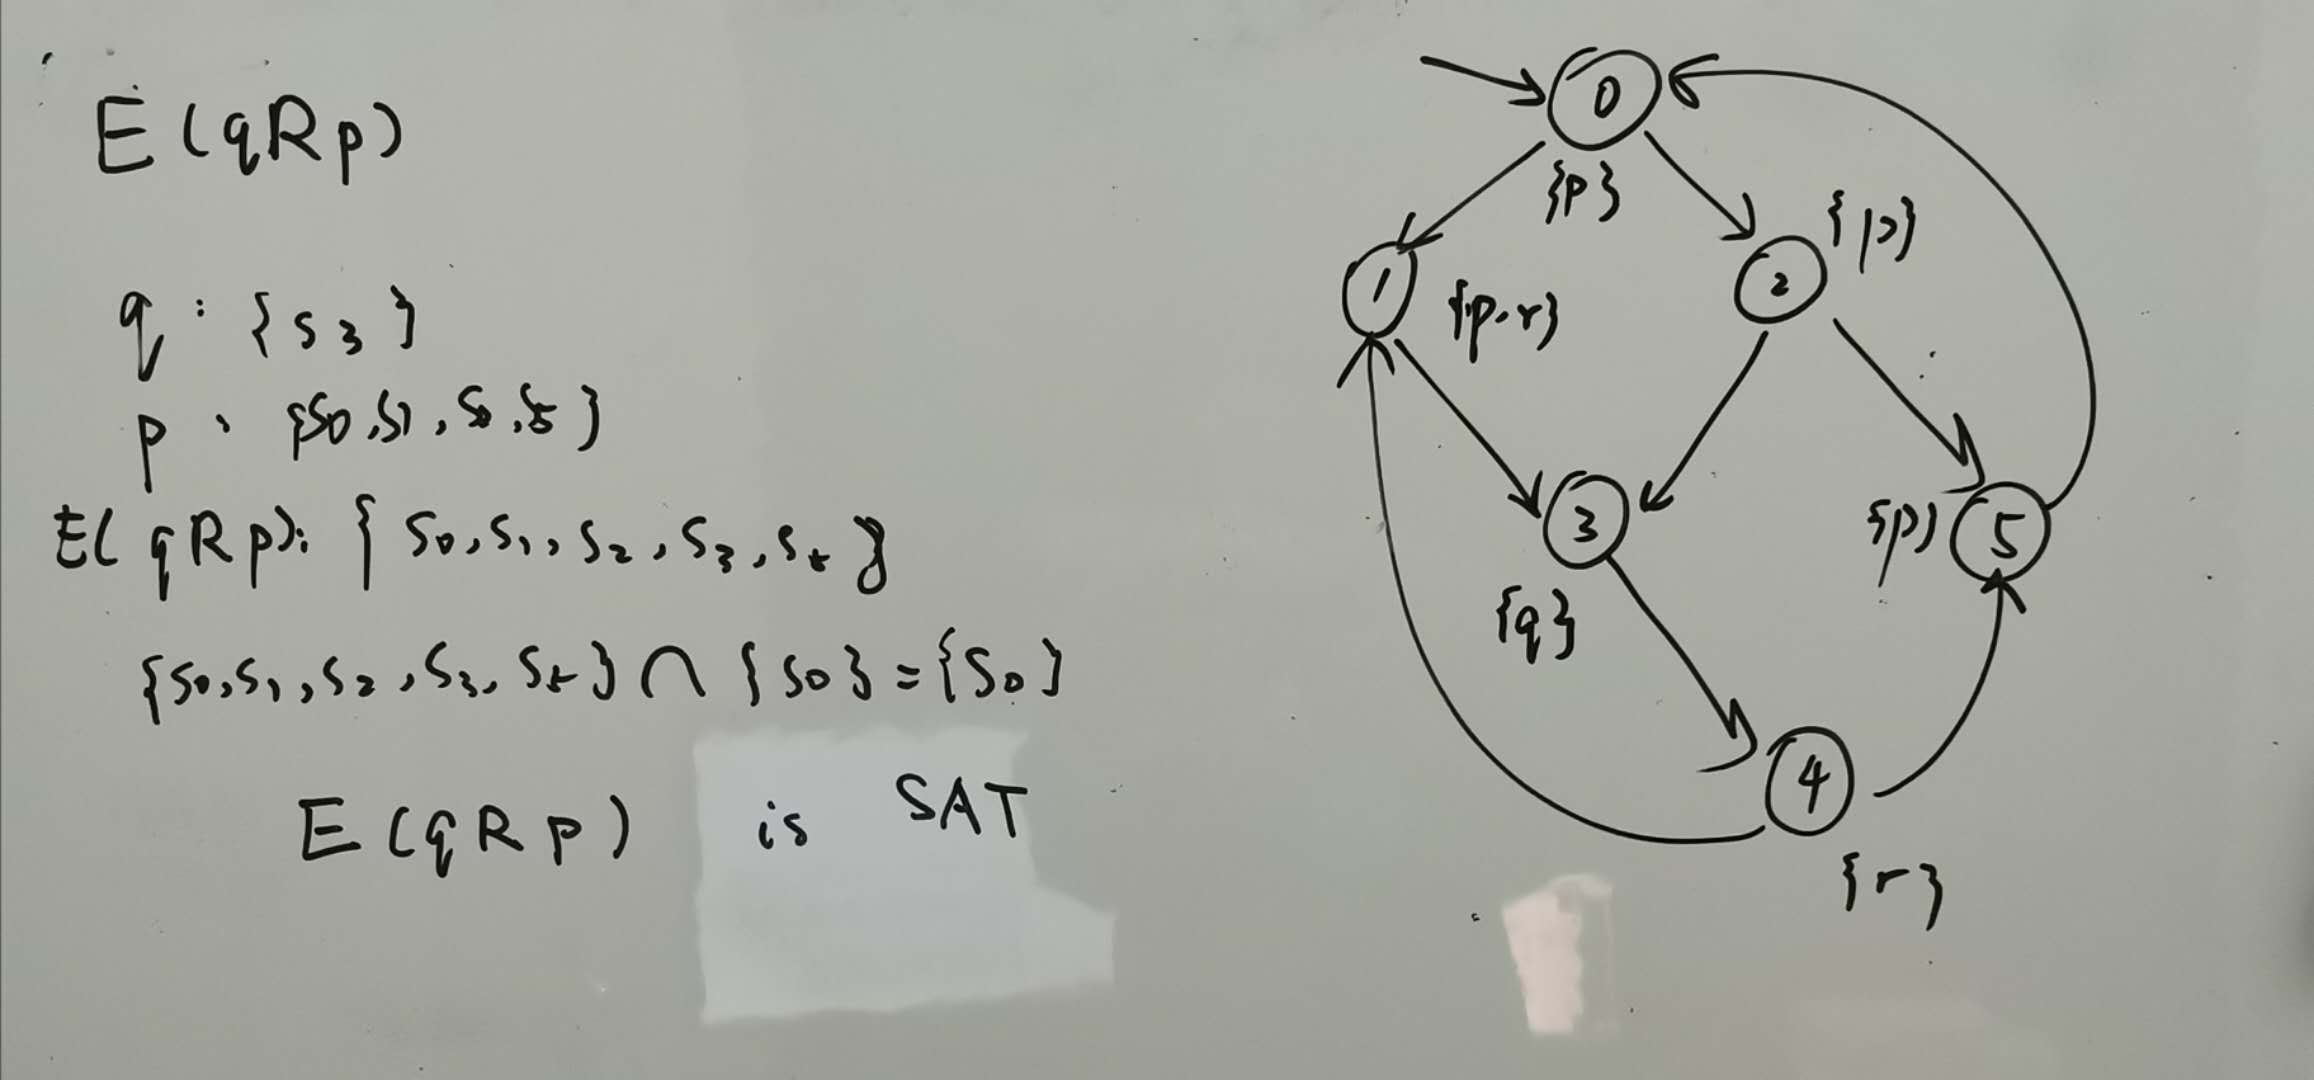
\includegraphics[scale=0.12]{7.jpg}

第三个性质:
不满足$(s_0 s_2 s_5)^\omega$这条路径是反例。


\item 增加公平约束:
答案:否,否,是

\item 选择第一种类型的性质。

$\textbf{E}(p\textbf{ U }q)$.

算法:对于每一个初始状态,做深度优先搜索,找到模型中的lasso,并且验证这个lasso的stem和loop是否满足$p\textbf{ U }q$的路径约束,并且对于lasso的loop上的状态,需要存在一个满足公平性质的状态。
如果有这样的lasso则返回SAT,否则返回UNSAT。
\end{enumerate}
\end{enumerate}


\end{document}